\section{Libreria Unity} \label{libreria_unity}

In questa sezione viene descritta la libreria realizzata per Unity mostrando la sua struttura e le sue componenti.

\subsection{Struttura}

\begin{figure}[H]
\centering
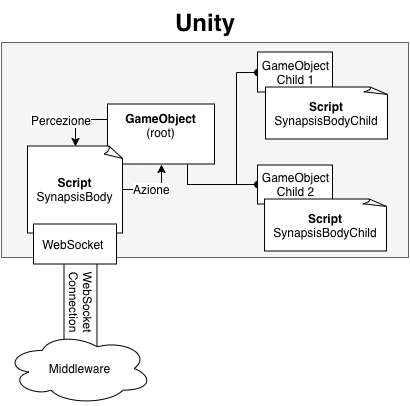
\includegraphics[width=0.7\textwidth]{figures/struttura_libreria_unity.png}
\caption{Struttura libreria per Unity}
\label{struttura_libreria_unity}
\end{figure}

L'immagine \ref{struttura_libreria_unity} mostra gli elementi che compongono la libreria realizzata per Unity.

\subsection{Script Synapsis}

\begin{figure}[H]
\centering
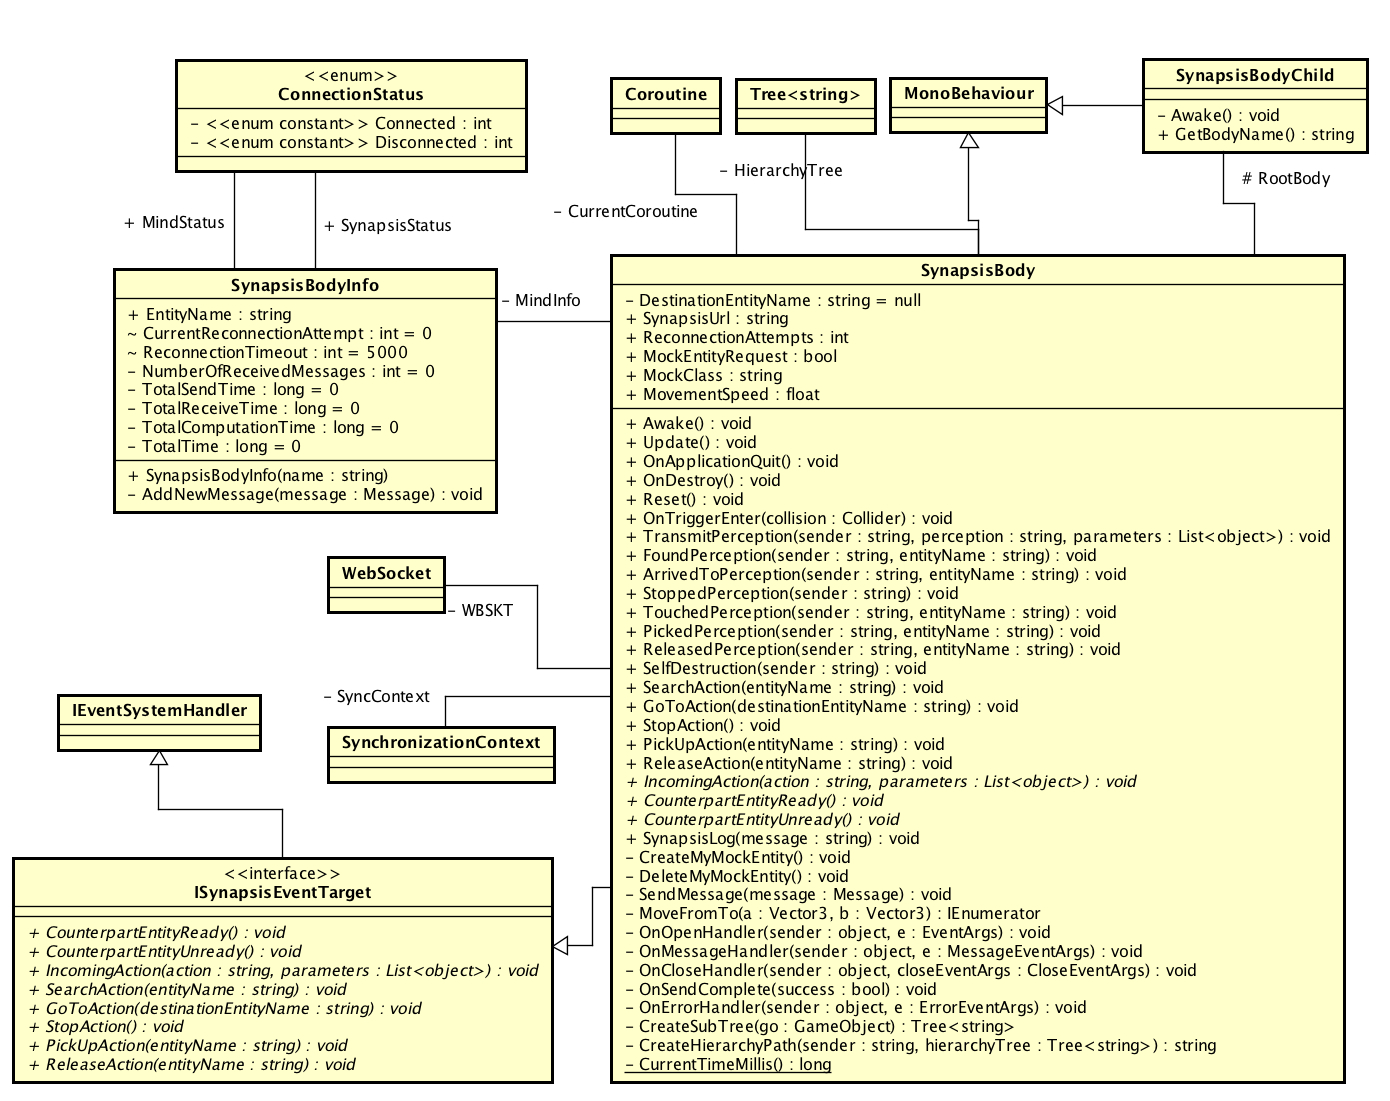
\includegraphics[width=\textwidth]{figures/diagramma_classi_script.png}
\caption{Diagramma delle classi della libreria per Unity}
\label{classi_libreria_unity}
\end{figure}

Il componente centrale della libreria per Unity è lo script \textit{SynapsisBody} che estende \textit{MonoBehaviour}, classe principale di Unity per definire comportamenti e caratteristiche dinamiche dei GameObject. Un qualsiasi GameObject che utilizza questo script è definibile come entità di tipo "corpo".

\medskip

Ad ogni GameObject a cui viene collegato uno script che estende SynapsisBody vengono richieste le componenti Collider \cite{unity_collision} e Rigibody \cite{unity_rigidbody} utilizzate per rendere il GameObject sensibile alle collisioni, informando automaticamente la mente tramite percezione.

\subsection{Funzionalità disponibili}
I seguenti metodi, presenti nello script \textit{SynapsisBody} sono a disposizione dello sviluppatore per inviare percezioni alla controparte \textbf{mind}.
\begin{itemize}
    \item TransmitPerception(sender, perception, params) --> invia alla controparte una percezione generica con parametri collegati;
    \item FoundPerception(sender, entityName) --> invia alla controparte la percerzione "found" e come parametro il nome dell'entità trovata. Viene automaticamente inviata in risposta ad un'azione "search" (precedentemente inviata dalla mente)
    \item ArrivedToPerception(sender, entityName) --> invia alla controparte la percezione "arrived\_to" e come parametro il nome dell'entità a cui si è arrivati. Viene automaticamente inviata in riposta ad un'azione "go\_to" (precedentemente inviata dalla mente)
    \item StoppedPerception(sender) --> invia alla controparte la percezione "stopped". Viene automaticamente inviata in riposta ad un'azione "stop" (precedentemente inviata dalla mente)
    \item PickedPerception(sender, entityName) --> invia alla controparte la percezione "picked" e come parametro il nome dell'entità prelevata. Viene automaticamente inviata in riposta ad un'azione "pick\_up" (precedentemente inviata dalla mente)
    \item ReleasedPerception(sender, entityName) --> invia alla controparte la percezione "released" e come parametro il nome dell'entità rilasciata. Viene automaticamente inviata in riposta ad un'azione "release" (precedentemente inviata dalla controparte mente)
    \item TouchedPerception(sender, entityName) --> invia alla controparte la percezione "touched" e come parametro il nome dell'entità toccata. Viene automaticamente inviata se il GameObject è dotato delle componenti "Rigibody" e "Collider".
\end{itemize}

Il metodo \textit{TransmitPerception} rappresenta la funzionalità più modulabile per inviare una generica percezione alla mente, mentre i restanti metodi sono stati definiti perchè rappresentano azioni comuni a molti scenari simili al caso di studio preso in esempio (Sezione \ref{caso_studio}).

\subsection{Gerarchia di oggetti complessi}

Sviluppando progetti su Unity, si fa largo uso di gerarchie \cite{unity_hierarchy} per realizzare oggetti complessi. Per evitare l'utilizzo di un collegamento WebSocket per ogni componente dell'oggetto complesso si è deciso di limitare concettualmente alla testa (root) dell'oggetto il collegamento alla mente.

\medskip

\'E stato realizzato uno script, estendibile, che permette anche alle sottoparti (child) di poter inviare percezioni alla mente, mantenendo l'informazione gerarchica valida e inviata assieme al messaggio.

\lstinputlisting[caption=SynapsisBodyChild script,language={[Sharp]C}]{code/SynapsisBodyChild.cs}

Per mantenere la struttura gerarchica valida, viene generata una struttura ad albero dove la radice (root) conterrà il nome del GameObject collegato allo script e, automaticamente, viene popolato il sottoalbero seguendo la struttura gerarchica di Unity.

\medskip

Ad ogni messaggio inviato alla controparte (mind) viene generato il path del GameObject che richiedere l'invio della percezione mappata in una stringa simile alla seguente: \textit{"nomeGORadice.nomeGOFiglio.nomeGOSottofiglio"}

\lstinputlisting[caption=Controllo gerarchia script,language={[Sharp]C}]{code/Gerarchia.cs}

Ad esempio, nel caso di invio di una percezione da parte di un GameObject "mano", figlio di un GameObject complesso chiamato "robot", il nome finale del mittente sarà "robot.mano".

\subsection{Inserimento WebSocket nel Event Loop di Unity}

Il modello computazionale presente su Unity è di tipo Event Loop: questo significa che tutti gli elementi presenti nella scena sono vincolati ad uno specifico lifecycle (Immagine \ref{unity_lifecycle}).

\begin{figure}[H]
\centering
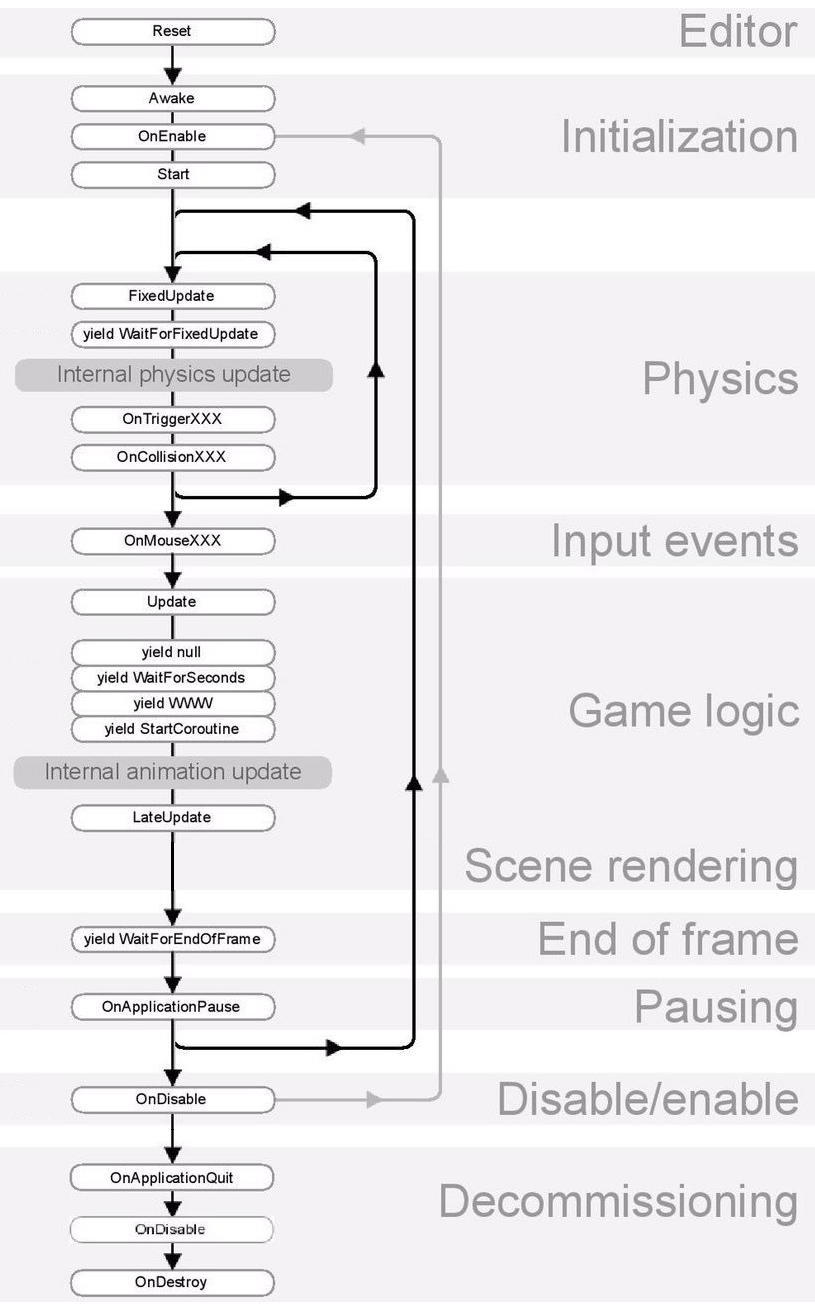
\includegraphics[width=0.9\textwidth]{figures/Unity_lifecycle.jpeg}
\caption{Unity Lifecycle}
\label{unity_lifecycle}
\end{figure}

Per interagire internamente tra i componenti, Unity mette a disposizione delle API definite come "Event System"\cite{unity_event_system} con le quali è possibile inviare eventi agli oggetti nell'applicazione in base all'input, che si tratti di tastiera, mouse, tocco o input personalizzato.

\medskip

La tecnologia di comunicazione, utilizzata per far ricevere informazioni (azioni) al corpo, ha portato a servirsi del sopra citato "Event System" di Unity. Questo perchè il canale WebSocket viene computazionalmente istanziato in un processo separato rispetto al normale lifecycle; inoltre perchè la politica presente in Unity non autorizza all'accesso diretto di thread separati a tutto ciò che è istanziato sul Main Thread\footnote{Thread principale di Unity}.

\lstinputlisting[caption={ISynapsisEventTarget},language={[Sharp]C}]{code/ISynapsisEventTarget.cs}

Per questo motivo è stato fatto uso dell'interfaccia \textit{IEventSystemHandler}, disponibile nelle API di Unity, per realizzare l'interfaccia \textit{ISynapsisEventTarget} attraverso la quale è possibile definire quali metodi sono utilizzabili anche da thread secondari. 

\medskip

Questa interfaccia viene implementata dallo script \textit{SynapsisBody}, così, nel momento in cui il middleware invia un messaggio, il processo contenente il canale WebSocket è in grado di invocare il relativo metodo (azione).